
The four \glspl{GDSM}s developed by the \gls{UFD} campaign facilitate sensitivity 
analysis of the long-term post-closure performance of geologic repositories in 
generic media with respect to various key processes and parameters 
\cite{clayton_generic_2011}. Processes and parameters expected to be influential to repository 
performance  include the rate of waste form degradation, timing of waste package 
failure, and various coupled geochemical and hydrologic characteristics of the 
natural system including diffusion, solubility, and advection.

The results here provide an overview of the relative importance of processes 
that affect the repository performance of simplified generic disposal 
concept in clay. This work is not intended to give an assessment of the performance of a 
disposal system. Rather, it is intended to  
generically identify properties and parameters expected to influence repository 
performance in a saturated, homogeneous geologic envrionment.


\section{Approach}

% used existing gdsms 
This analysis utilized the \gls{GDSM} developed by the \gls{UFD} campaign to 
represent a clay repository concept. The \gls{GDSM} performs detailed 
calculations of radionuclide transport within a clay repository concept \cite{clayton_generic_2011}.  

% describe their features 
The radionuclide transport calculations
are performed within the GoldSim simulation platform. GoldSim is a commercial 
simulation environment 
\cite{golder_associates_goldsim_2010, golder_associates_goldsim_2010-1}. 
Probabilistic elements of the GoldSim modeling framework enable the models to 
incorporate simple probabilistic \gls{FEPs} that affect repository performance 
including waste package failure, waste form dissolution, and an optional 
vertical advective fast pathway \cite{clayton_generic_2011}. 

The GoldSim framework and 
its contaminant transport module provide a simulation framework and 
radionuclide transport toolset that the \glspl{GDSM} have utilized to 
simulate chemical and physical attenuation processes including radionuclide 
solubility, dispersion phenomena, and reversible sorption 
\cite{golder_associates_goldsim_2010, golder_associates_goldsim_2010-1}. 

% WMN suggested deleting this, cells are only one part of the goldsim framework
%Cells within GoldSim represent components of the waste disposal system and
%are linked by diffusive, advective, precipitated, direct, or  otherwise filtered
%mass transfer links. 

 

\section{Mean of the Peak Annual Dose}

In this analysis, repository performance is quantified by radiation dose to a 
hypothetical receptor. Specifically, this sensitivity analysis focuses 
on parameters that affect the mean of the peak annual dose.  The mean of the 
peak annual dose,

\begin{align} \label{MoP}
  D_{MoP,i} &= \frac{\sum_{r=1}^{N}{\max\left[\left.D_{r,i}(t)\right|_{\forall t}\right]}}{N}
  \intertext{where}
  D_{MoP,i} &= \mbox{mean of the peak annual dose due to isotope i} [mrem/yr]\nonumber\\
  D_{i}(t) &= \mbox{annual dose in realization r at time t due to isotope i } [mrem/yr]\nonumber\\
  N &= \mbox{Number of realizations, } \nonumber
\end{align}

is a conservative metric of repository performance. The mean of the 
peak annual dose should not be confused with the peak of the mean annual dose,

\begin{align} \label{PoM}
  D_{PoM,i} &= \max\left[{\frac{\sum_{r=1}^{N}{\left.D_{r,i}(t)\right|_{\forall t}}}{N}}\right]\\
            &= \mbox{peak of the mean annual dose due to isotope i } [mrem/yr].\nonumber
\end{align}

The mean of the peak annual dose rate given in equation \eqref{MoP} 
captures trends as well as the peak of the mean annual dose rate given 
in equation \eqref{PoM}. However, the mean of the peaks metric, $D_{MoP,i}$, was 
chosen in this analysis because it is more conservative since it is able to 
capture temporally local dose maxima and consistently reports higher dose values 
than the peak of the means, $D_{PoM,i} $.




\section{Sampling Scheme}

The multiple barrier system modeled in the clay \gls{GDSM} calls for a 
multi-faceted sensitivity analysis. The importance of any single component or 
environmental parameter must be analyzed in the context of the full system of 
barrier components and environmental parameters. Thus, this analysis has 
undertaken an analysis strategy to develop a many dimensional overview of the 
key factors in modeled repository performance. 

To address this, both individual and dual parametric studies were performed. 
Individual parameter studies varied a single parameter of interest in 
detail over a broad range of values. Dual parameter sensitivity studies were 
performed for pairs of parameters expected to exhibit some covariance. For 
each parameter or pair of parameters, forty simulation 
groups varied the parameter or parameters within the range considered. Example 
tables of the resulting forty simulation groups for  individual 
and dual parametric study configurations appear in Tables \ref{tab:indivgroups} 
and \ref{tab:dualgroups} respectively.

\begin{table}[h!]
\centering
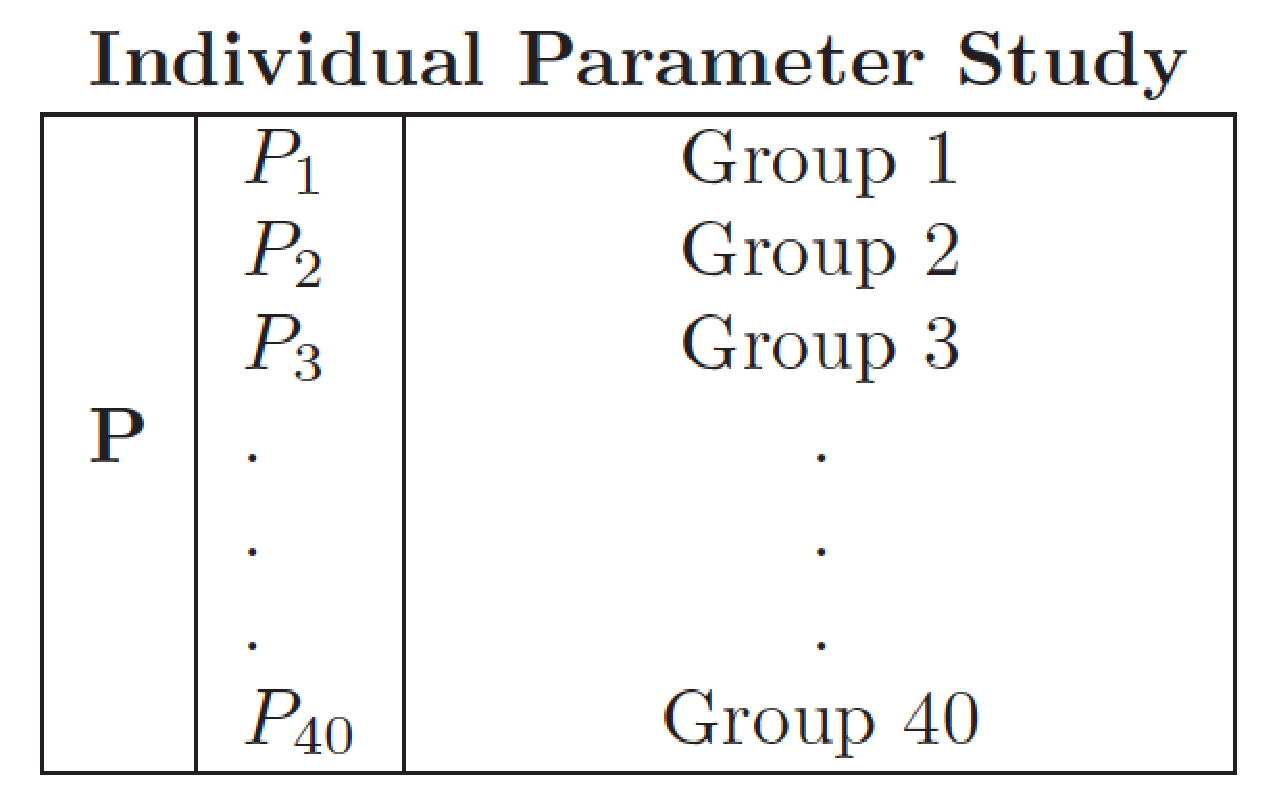
\includegraphics[width=0.3\textwidth]{./chapters/nuclide_sensitivity/indiv_groups.eps}
\caption{For an individual one group of 100 realizations was run for each 
each discrete value, $P_{i}$, within the range considered for $P$.}
\label{tab:indivgroups}
\end{table}

\begin{table}[h!]
\centering
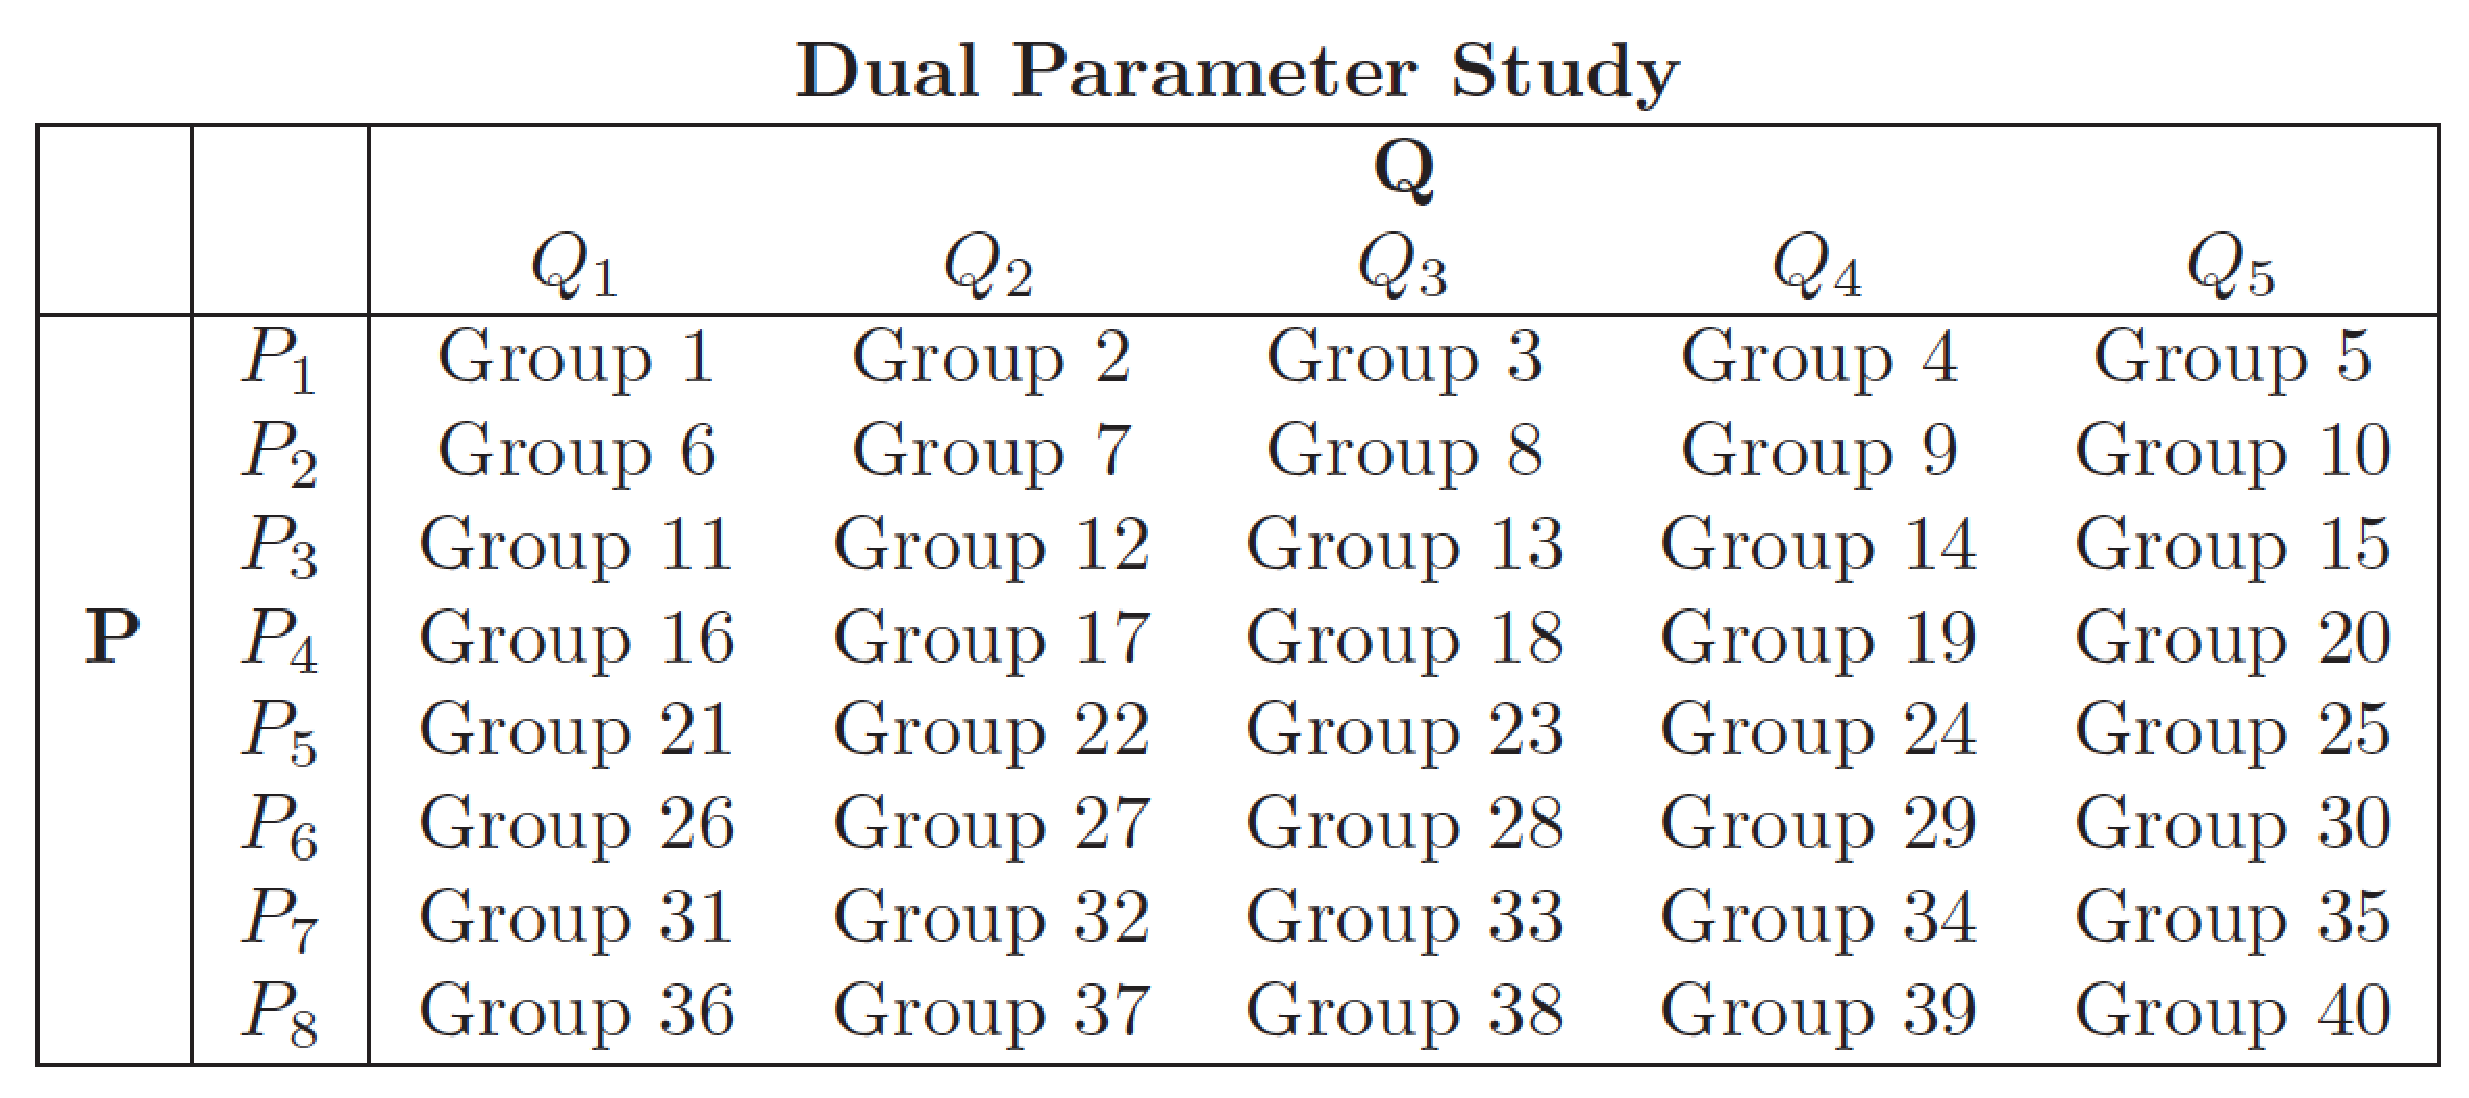
\includegraphics[width=0.6\textwidth]{./chapters/nuclide_sensitivity/dual_groups.eps}
\caption{The simulation groups for a dual simulation sample each parameter 
within the range over which it was considered.}
\label{tab:dualgroups}
\end{table}

For each simulation group, a 100 realization simulation was completed. Each
realization held the parameters being analyzed as constant and sampled 
stochastic values for uncertain parameters not being studied.  A sampling scheme 
developed in previous generic disposal media modeling was implemented in this 
model in order to ensure that the each 100 realization simulation sampled 
identical values for uncertain parameters \cite{clayton_generic_2011, 
nutt_generic_2009}.  

In order to independently analyze the dose contributions from radioisotope 
groups, four cases,

\begin{itemize}
  \item Americium and its daughters,
  \item Plutonium and its daughters,
  \item Uranium and its daughters,
  \item Neptunium, its daughters, and fission products
\end{itemize}

were run independently. This allowed an evaluation of the importance of daughter 
production from distinct actinide chains. 
